O meu plano de desenvolvimento pessoal, passa por obter mais formação e apreender com pessoas com mais experiência em diversas áreas, que é exatamente o que estou a fazer frequentando o curso de Engenharia Eletrotécnica e de Computadores no \textcolor{gray}{I.S.E.P}.\\
Esta disciplina em particular é uma forma de poder enriquecer minhas competências de Gestão, e as matérias abordadas que compõem o \textcolor{blue}{Comportamento Organizacional}, que são bastantes.
\begin{figure}[H]
	%\centerline
	\begin{minipage}{\linewidth}
		\centering
		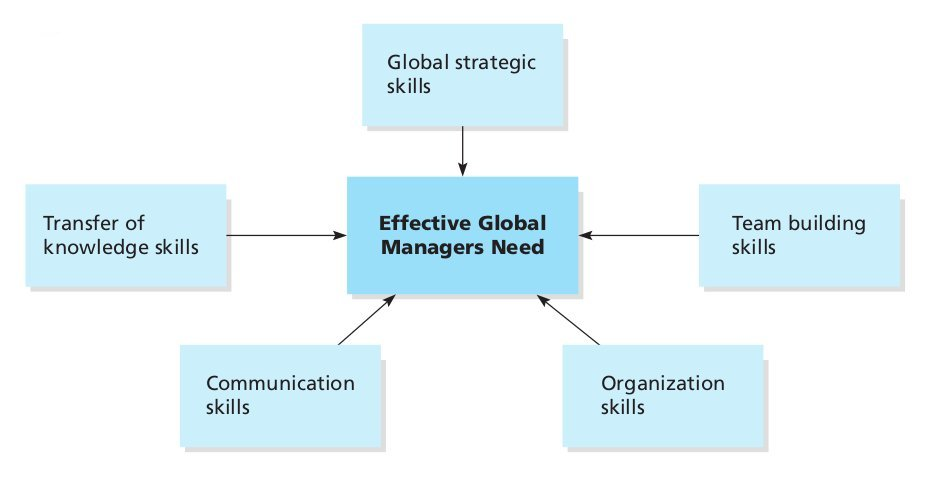
\includegraphics[scale=0.3]{"./image/Skills/Managerial Skills for the Global Marketplace.jpg"}
	\end{minipage}
	\caption{Competências de Gestão. \cite{book_6}}
\end{figure}






\begin{comment}
a) Realizar um diagnóstico de competências pessoais;\\
b) Definir objetivos de carreira;\\
c) Definir as competências que considere que no futuro lhe permitirão atingir os referidos objetivos;\\
d) Definir um plano de desenvolvimento para as competências anteriormente selecionadas.
\end{comment}